\section{System Overview}
    \subsection{Intel Aero Compute Board}
    The Intel® Aero Compute Board is a purpose-built, unmanned aerial vehicle (UAV) developer kit powered by a quad-core Intel® Atom™ processor and geared toward UAV developers, researchers, and enthusiasts. It features abundant storage capabilities, 802.11ac Wi-Fi, support for multiple cameras including the Intel® RealSense™ camera (R200), industry standard interfaces, and reconfigurable I/O to facilitate connecting to a broad variety of drone hardware subsystems. The compute board ships with open-source Yocto Project for embedded Linux systems and offers sample applications and APIs for flight and vision interfaces, reducing hurdles for developers of sophisticated drone applications.

    This development platform is intended to be modified by developers according to their professional judgment. Intel has not established operating limitations for the kit or tested any configurations other than the base configuration that is shipped as configured from the factory.
    \begin{table}[h!]
      \centering
      \setlength\extrarowheight{-0pt}
      \begin{tabular}{ l>{\scriptsize}c>{\scriptsize}l }
        %\cmidrule(r){2-3}
        \multirow{12}{*}{\begin{minipage}{.6\textwidth}
          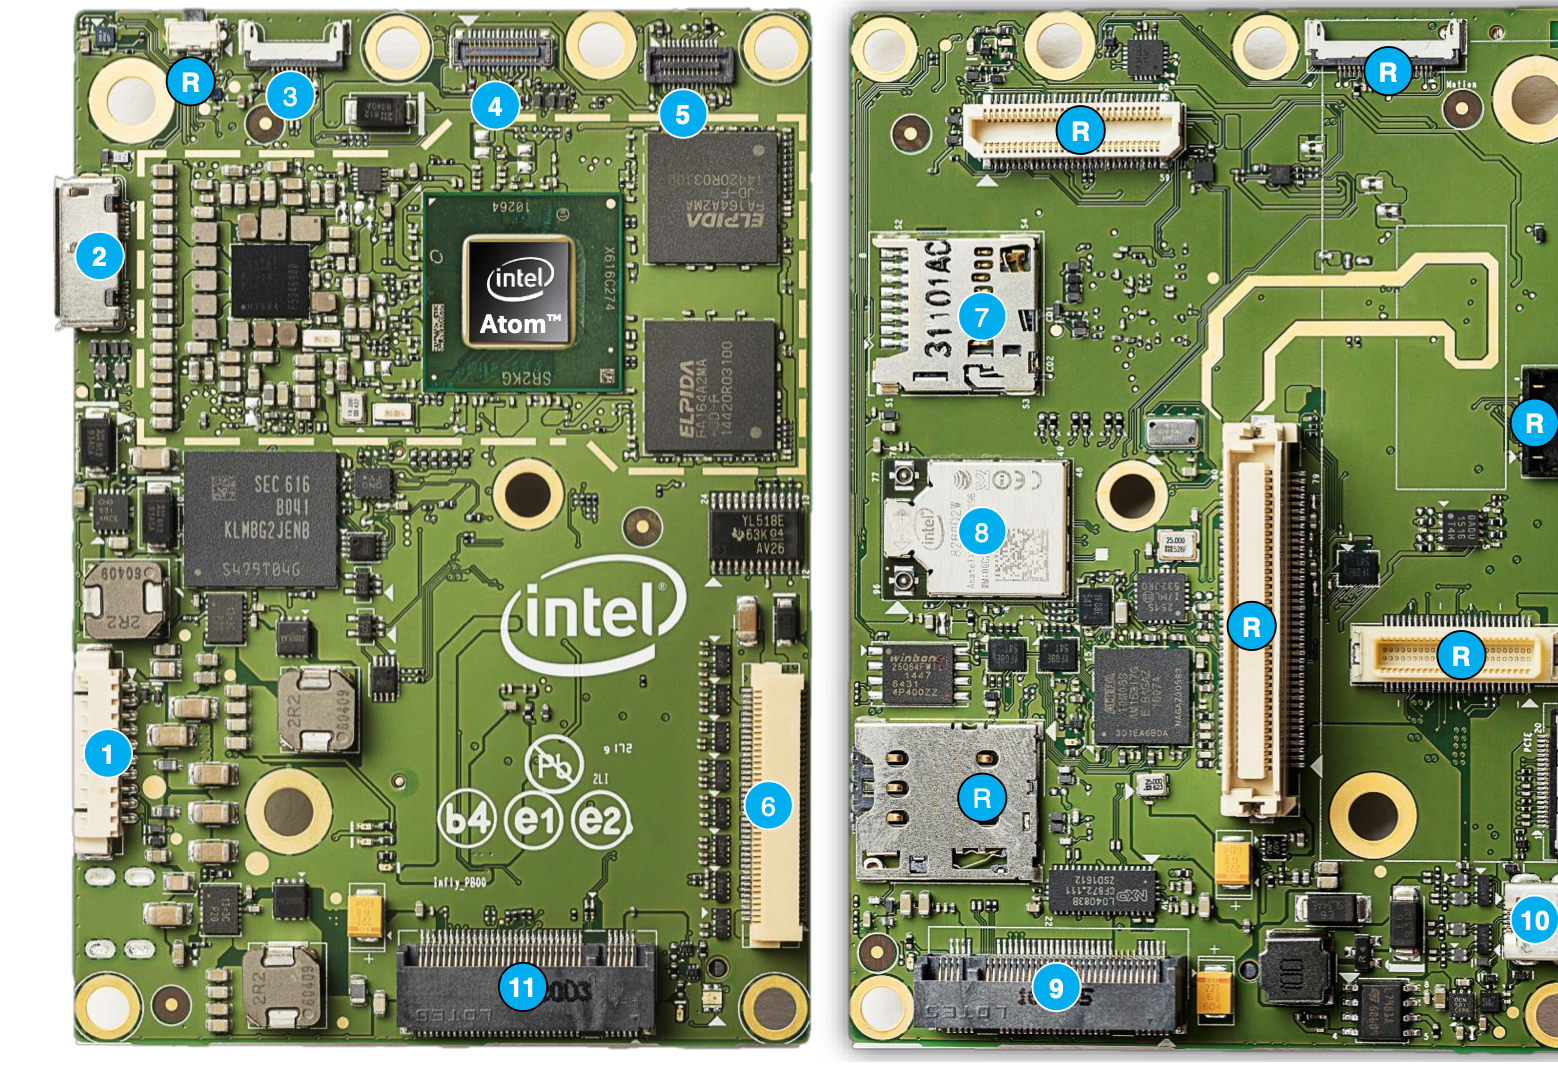
\includegraphics[width=\linewidth]{templates/images/chapter05/intel-aero-compute-board.png}
        \end{minipage}}&1&Power connector\\
        &2&USB 3.0 OTG \\
        &3&Interface for Intel RealSense camera \\
        &4& MIPI interface for HD camera \\
        &5& MIPI interface for VGA camera \\
        &6& 80 pin flexible I/O (I2C,SPI,UART) \\ 
        &7&microSD Memory Card slot\\
        &8&Intel Dual Band Wireless-AC\\
        &9&PCIe x1 M.2 Interface\\
        &10&Micro HDMI port\\
        &11&NGFF M.2 connector\\
        &R&RESERVED for future use\\
        %\cmidrule(r){2-3}%\hline
      \end{tabular}
      \caption{Intel Aero Compute Board Connector Layout. Source: \cite{intel-aero-combrd}}
      \label{tbl:aero-board-layout}
    \end{table}
\newpage 
    All signals from the Aero Flight Controller (except the SDIO interface and CAN bus) are routed through the MAX10 FPGA to the IO Expansion connector. The pin assignments can be found in the Hardware Features and Usage document. The FPGA is in charge of routing the IOs between the (*SoC) System-on-Chip and the motors plus flight controller. The pin functions from the Aero Flight Controller may vary according to the STM32's pinmux configuration. The Flight Controller hardware contains a CAN bus transceiver.
    
    \begin{figure}[H]
        \centering
        \begin{minipage}{0.45\textwidth}
            \centering
            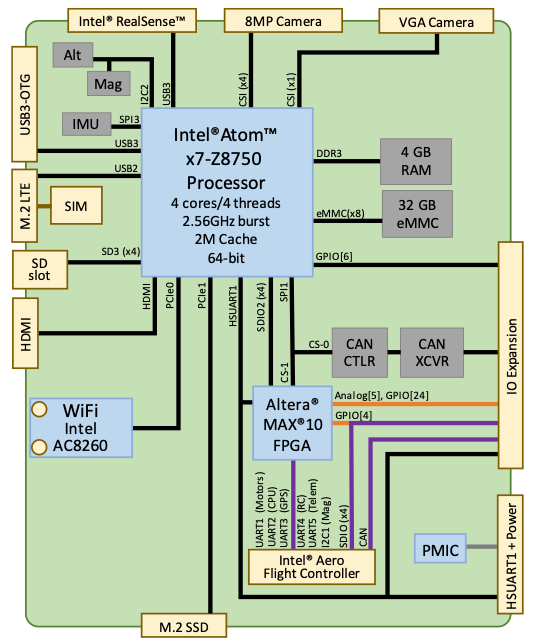
\includegraphics[width=\textwidth]{templates/images/chapter05/compute-board-diagram-nbw.png} % first figure itself
            %\caption{first figure}
        \end{minipage}%\hfill
        \begin{minipage}{0.4\textwidth}
            \centering
            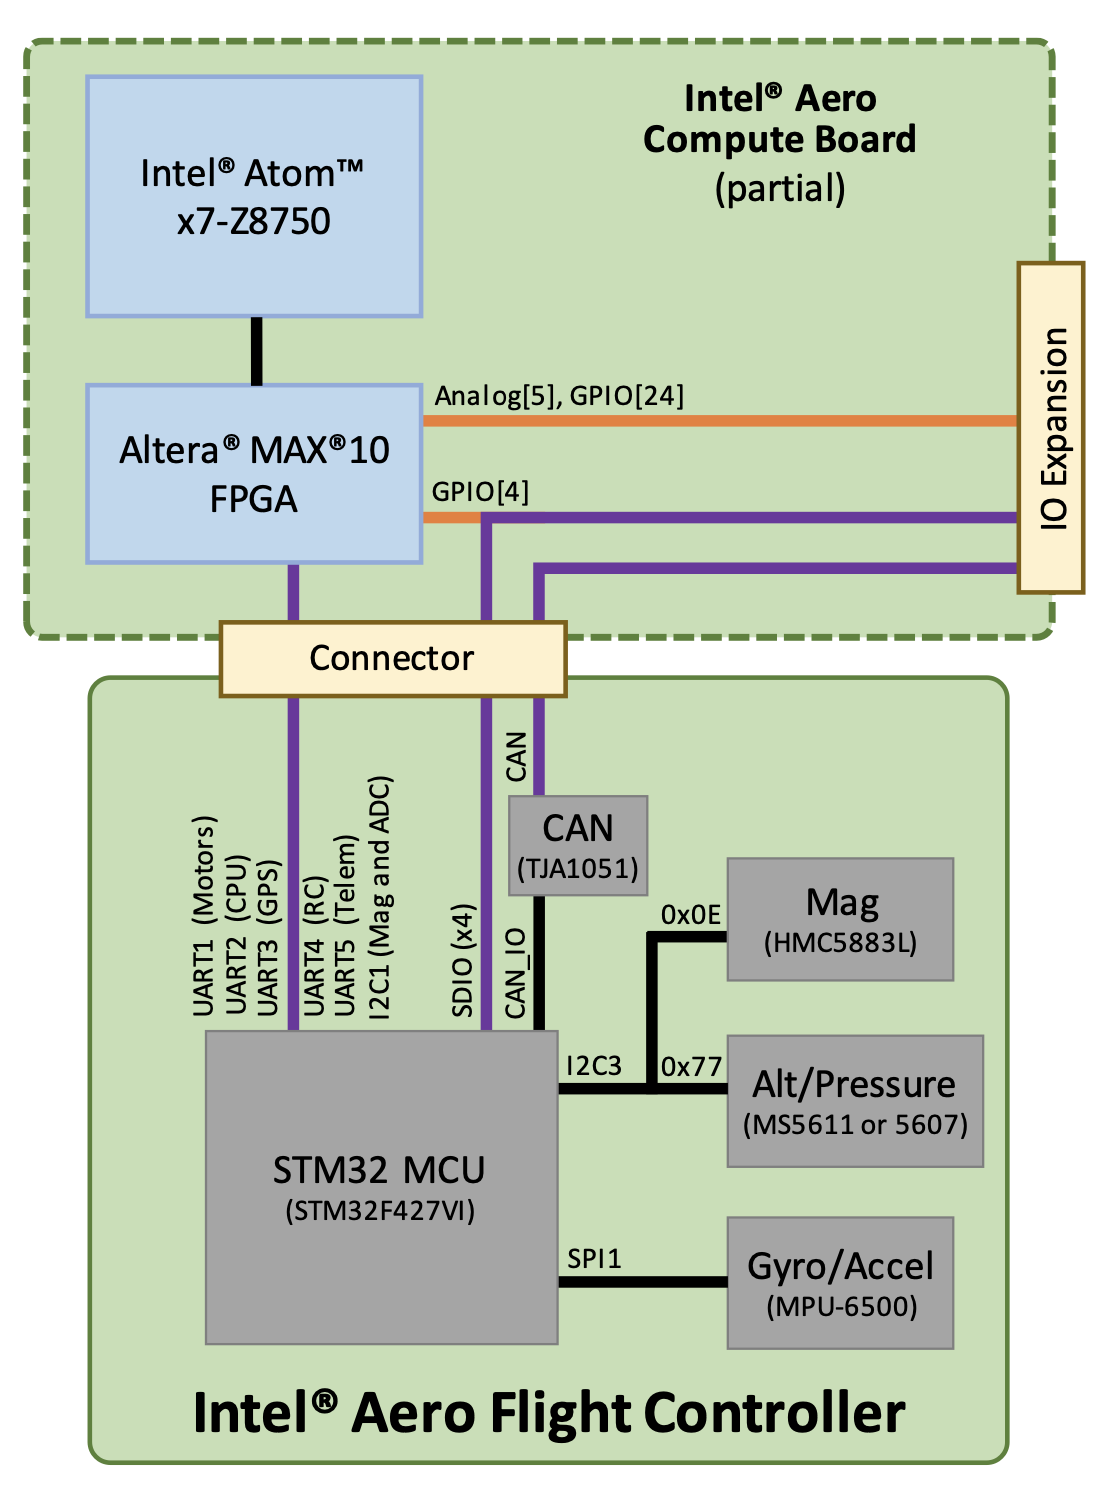
\includegraphics[width=\textwidth]{templates/images/chapter05/flight-controller-diagram-nbw.png} % second figure itself
            %\caption{second figure}
        \end{minipage}
        \caption{Respective module block diagrams. Source: \cite{intel-aero-combrd}}
    \end{figure}
    
    %[*Intel® Aero Compute Board: Hardware Features and Usage Rev 1.5.2,https://www.intel.com/content/dam/support/us/en/documents/drones/development-drones/intel-aero-compute-board-guide.pdf]
\newpage
    By default, Intel Aero board and Intel Aero Ready To Fly kit are delivered with a Yocto Project build already flashed. Yocto project is an open source set of tools for embedded professionals. The UEFI BIOS is maintained by InsydeH20.\footnote{Since September 04, 2019, Intel has discontinued the Intel Aero Platform for UAVs. Forum-based support (Intel Community) for Intel Aero products is available until June 15, 2019. There are no further software updates planned for the Intel Aero Platform for UAVs. All documentation resources for the Intel Aero products will be available to the Intel Aero developer community until February 15, 2022. Files licensed under open source licenses will continue to be available in binary and source code on GitHub.} This Yocto build is preconfigured and highly customized for Intel Aero. In parallel to this Intel supported Yocto image, full native Ubuntu with Intel drivers is available as user installation.
    
    For our use-case a huge effort was dedicated in order to fine-tune the appropriate configuration of hardware and software as to not jeopardize the reliability of the system. More specifically, it was found that under no circumstances any other version of Ubuntu Linux 16.04.3 should not be installed, for the sole reason that the system would cease to boot entirely. Additionally, any updates could cause instabilities, including important security patches. For this reason, the software stack is considered highly insecure in terms of being up-to-date with current Linux distributions and should not be operated on public-facing infrastructures and is intended only for demonstration purposes. 
    
    Facing a choice between the two Linux distributions available for the platform, namely a pre-configured Yocto Project supplied by Intel with the necessary packages for conventional applications or the desktop version of Ubuntu 16.04, versatility was a deciding factor. Although more lightweight and use-case specific, Yocto does not come with a package manager, with the only option being a re-compilation of the system image using so-called "recipes", something that would be extremely time consuming and with varialble results. For this reason, we opted for the commercially available Ubuntu distribution, placing additional care as to not diverge greatly from the basic configuration, apart from necessary packages for our use-case.
    
    \begin{figure}
        \centering
        \begin{minipage}{0.5\textwidth}
            \centering
            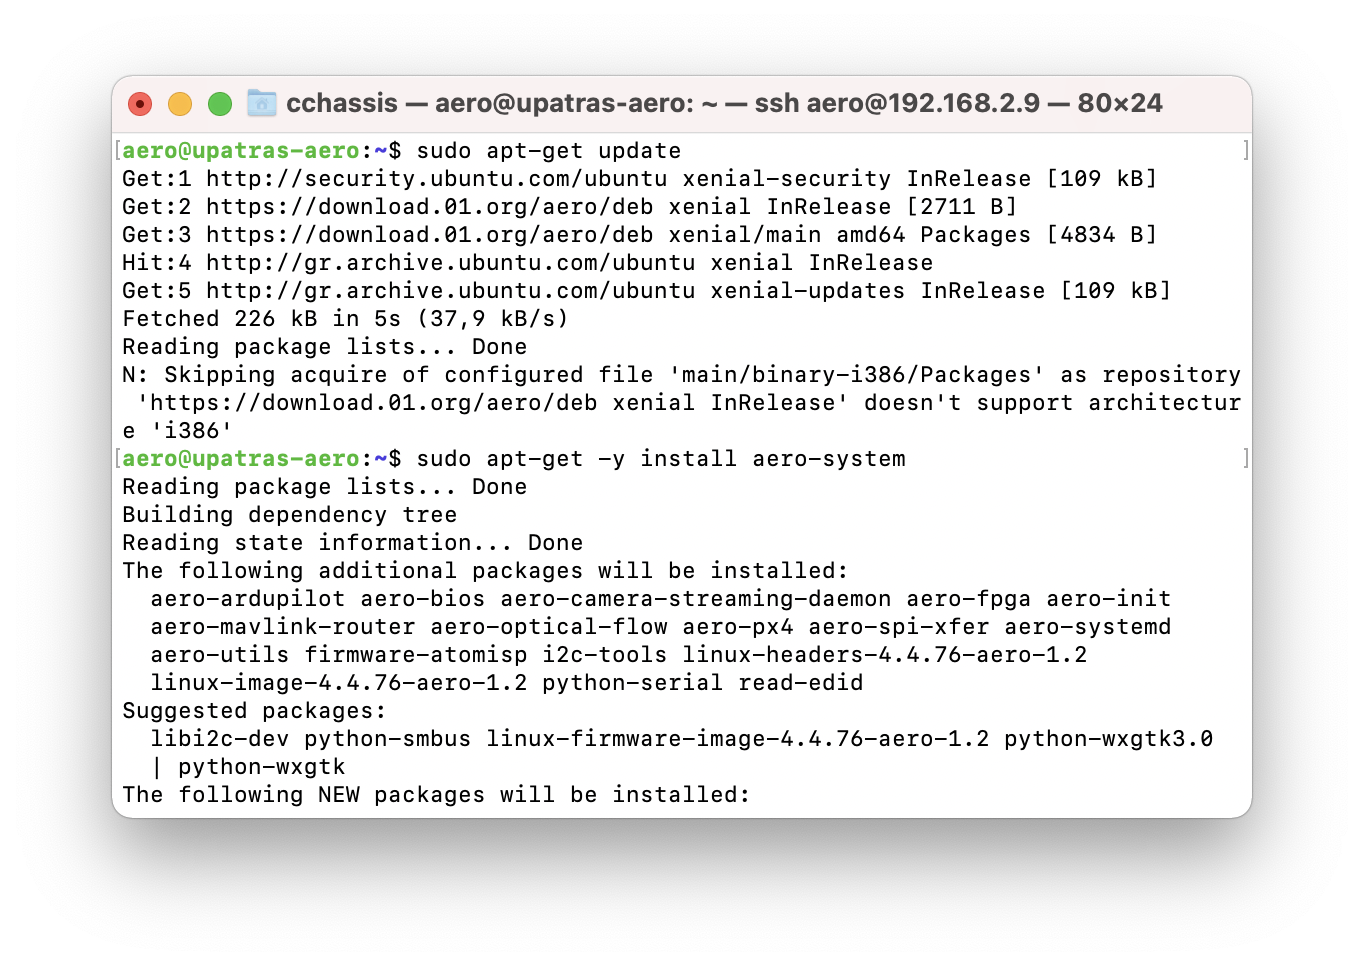
\includegraphics[width=\textwidth]{templates/images/chapter06/06-04-install-aero-system.png} % first figure itself
            %\caption{first figure}
        \end{minipage}\hfill
        \begin{minipage}{0.48\textwidth}
            \centering
            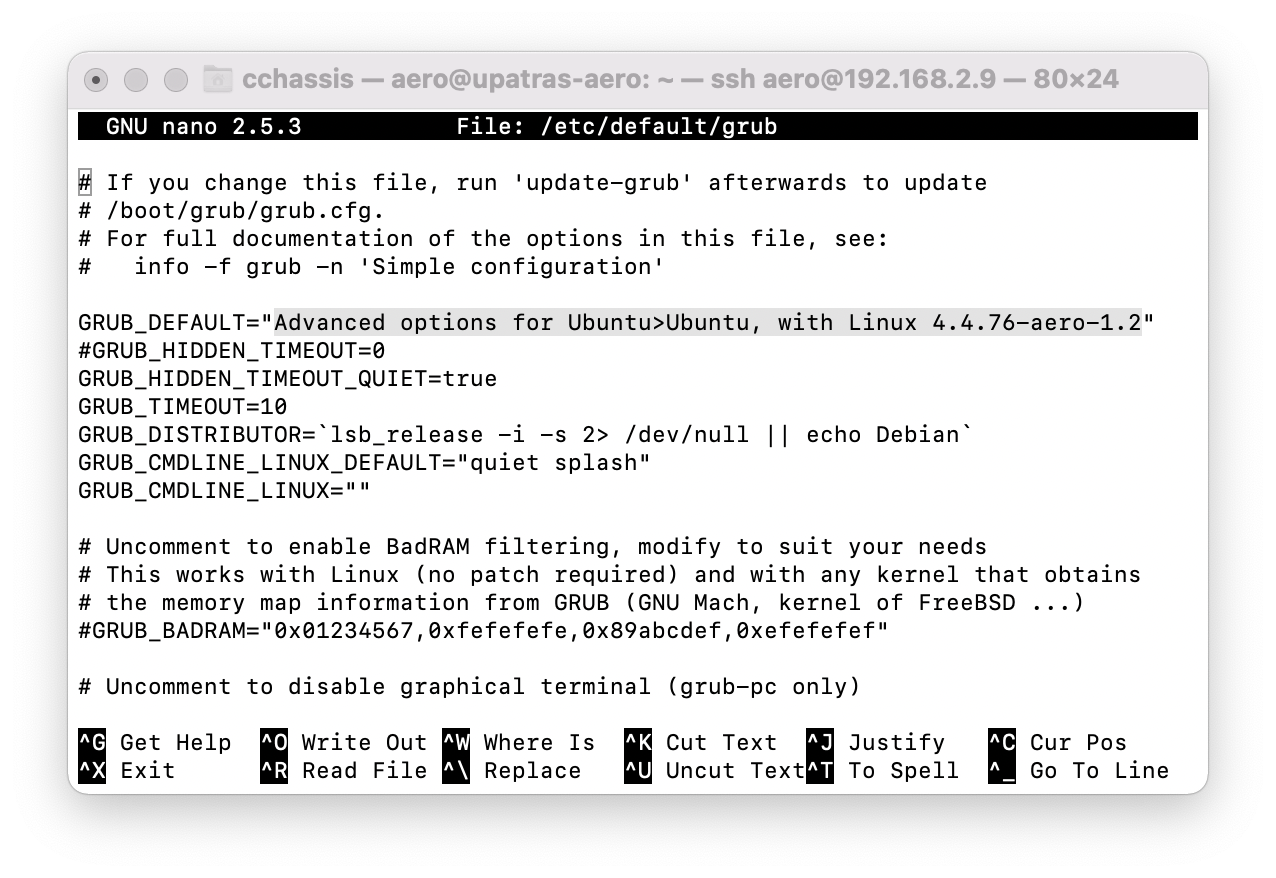
\includegraphics[width=\textwidth]{templates/images/chapter06/06-05-bnw.png} % second figure itself
            %\caption{second figure}
        \end{minipage}
        \caption{Downloading and setting correct kernel version.}
    \end{figure}

    \subsection{Flight Controller}
    Included in the Ready to Fly (RTF) kit, an STM32F427V autopilot board is responsible for hosting the Real Time Operating System (RTOS), under which the Autopilot Software Suite operates. The flight controller also hosts a variety of sensors responsible for vital vehicle operations such as a magnetometer and a compass, along with a plethora of connectivity for additional use-case specific modules. This specific module comes pre-installed on the aformentioned companion computer, attached via a proprietary connector. This raises some questions regarding the serviceability of the platform, since replacement parts are no longer available, but an external aftermarket flight controller can always be connected via a USB connection.
    
    Regarding the autopilot, the two most popular stacks were under consideration for this implementation, namely PX4 and Ardupilot, with the former being the ultimate choice. PX4 consists of two main layers: the flight stack which is an estimation and flight control system, responsible for the basic functionalities of any autonomous vehicle such as balancing and positional awareness and the middleware, which is a general robotics layer that can support any type of autonomous robot that consists primarily of device drivers for embedded sensors and communication with the external world (companion computer, Ground Control Stations, etc.).
    
    \subsection{Cameras}
    Placed in the front-facing side of the quadrotor assembly, the Intel® RealSense™ R200 module is a implements a long range, stereovision 3D imaging system that implements a variety of capabilities to be used accordingly. More specifically, it can provide color, depth, and infrared video streams. Depth video streams are like color video streams, except each pixel has a value representing the distance away from the camera instead of color information. It consists of an infrared laser projection system, two infrared and a full HD color imaging sensors. The depth video stream is generated with stereo vision technology assisted by the Infrared laser projector and the two infrared imaging sensors. Color data is provided by the full HD color imaging sensor.
    
    Due to the complexity of such device, additional effort has to be taken in order to ensure proper operation during the use-case scenario.
    
    Initially, a custom kernel must be booted in order for the various camera modules to be recognized appropriately. Following, the legacy branch of the RealSense R200 public repository must be configured on the Ubuntu 16.04.3 OS, where after successful initialization, three distinct video devices should be listed using the command  \verb|sudo v4l2-ctl --list-devices|.
    To check if the camera drivers are correctly installed, list the video devices with \verb|ls /dev/video*|
%https://github.com/intel-aero/meta-intel-aero/wiki/90-(References)-OS-user-Installation#checks
    
    
    \subsubsection{Third Party Cameras} %any 360 cameras w/ linux drivers?
    It is also possible to connect another camera for further use case expansions. What is imperative though is ensuring compatibility with existing IO ports on the Intel Aero compute board (SPI, CAN and USB are available) and linux driver support (typically UVC, USB Video Class). The camera is recognized as a UVC device, as expected. As before, run \verb|ls /dev/video*| to list the video devices. Use \verb|sudo v4l2-ctl --list-devices| to get the details about the camera-number association.
%https://github.com/intel-aero/meta-intel-aero/wiki/06-Cameras-and-Video#third-party-usb-cameras
    
    %\section{Software}


\newpage

    \subsection{Additional Software}
    
    Following proper setup of both the software and hardware aspects of the system, the next step is to ensure its key functionalities in order to operate within the use-case requirements. For this reason, two main software stacks need to be individually installed and configured, detailed below.
    
    \begin{figure}[H]
        \centering
        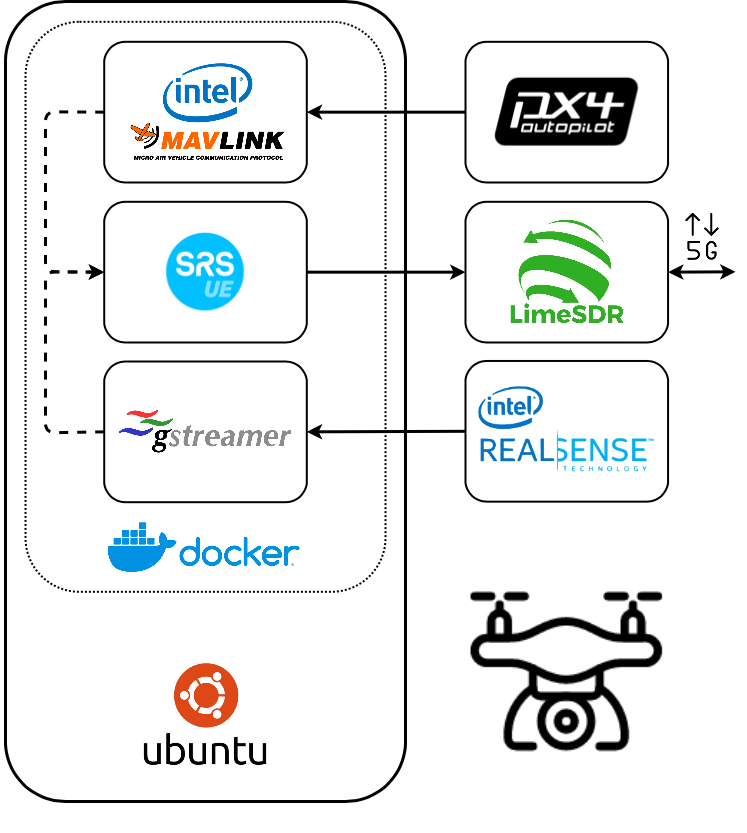
\includegraphics[width=0.9\textwidth]{templates/images/chapter05/vehicle-side-overview-2.png}
        \caption{Vehicle-side overview of the software sub-systems.}
        \label{fig:vehicle-side-sw}
    \end{figure} 
    
    \subsubsection{MAVLink-Router}
    
    MAVLink is a packet implementation for communicating drone messages, a popular interface for flight controllers such as PX4, Ardupilot and more. This was mainly used for Ground Control Stations (GCS) such as QGroundControl and Mission Planner, mainly for the command and control link. MAVLink follows a modern hybrid publish-subscribe and point-to-point design pattern: Data streams are published as topics while configuration sub-protocols such as the mission protocol or parameter protocol are point-to-point with retransmission. MAVLink is a binary telemetry protocol designed for resource-constrained systems and bandwidth-constrained links. The low level implementation of this protocol allows packets to be sent over UDP, TCP and serial interfaces with the exact same message format. Messages can be received over a serial connection and be forwarded to one or many UDP/TCP/serial connections. Telemetry data streams are sent in a multicast design while protocol aspects that change the system configuration and require guaranteed delivery like the mission protocol or parameter protocol are point-to-point with retransmission. Most services use the client-server pattern, such that the GCS (client) initiates a request and the vehicle (server) responds with data. Many existing solutions that provide network routability of MAVLINK packets exist, but the aforementioned MAVProxy, written in Python is relatively slow-performing%[System Engineering and Embedded Software Architecture WOrkshop | UAS@UCLA p.3 of 9 "MAVLink Messages and Routeing (CS118) - https://uasatuca.org/fields/workshops/controls]
    , thus unsuitable for real-time operation. Fortunately, alongside the commercial release of Intel Aero*, the company releaased a plethora of supporting applications, one of which is mavlink-router, written in C++%/ref{*}
    , with its implementation seems more appropriate for low-latency scenarios.
    
    Mavlink-router is an Intel open source project that routes MAVLink streams to specific endpoints, first implemented on the Intel Aero to handle communications with the companion computer. In addition to routing streams, mavlink-router has the ability to route MAVLink streams over a network. This can be done either manually, or through a configuration file.%Using mavlink-router to route MAVLink streams over the network[Jaeyoung Lim-august 25,2018-404warehouse-https://404warehouse.net/2018/08/25/using-mavlink-router-to-route-mavlink-streams/]

\newpage

    \begin{lstlisting}[caption=Example of a typical configuration file.]
[General - Mavlink-router serves on this TCP port]
TcpServerPort=5790
ReportStats=false
MavlinkDialect=auto

[TcpEndpoint Localhost]
Address = 127.0.0.1
Port = 25790
RetryTimeout=10
 
[UdpEndpoint Eavesdropping]
Mode = Eavesdropping
Address = 0.0.0.0
Port = 10000

[UdpEndpoint Endpoint]
Mode = Normal
Address = <ADDRESS>
Port = 11000

[TCPEndpoint LTE]
Address = XX.XX.XX.XX (replace with GCS ip) 
Port = 5760

Log=$HOME/log/flight-stack
LogMode=while_armed
    \end{lstlisting}

\newpage

    Mavlink-router's primary purpose as the name suggests, is to route MAVLink streams between endpoints. The normal usage of mavlink-router is to listen to a flight controller (usually on a serial or UDP port) and forward traffic to other endpoints. A UartEndpoint is defined to listen to a serial device, usually the flight controller. In this case, the flight controller is attached to the ttyS1 serial device of the OS. The mavlink stream can be routed to a UdpEndpoint or a TcpEndpoint of a specified address and port.
    In order to forward streams to Ground Control Stations the parameter \verb|Mode = Normal| needs to be specified. A very important feature is that commands can be sent to the Flight Controller Unit from said endpoints, allowing for complete remote operation over IP. MAVLinks lastly, can be broadcasted over an entire network, by configuring the Bcast address of said network. This proves useful if a VPN (or a network slice) is used as a dedicated network for controlling the drone. \verb|mavlink-router| also listens, by default, on port 5760 for TCP connections. Any connection there will also receive routed packets.

    Lastly, mavlink-router provides logging functions in which enables logging on the companion computer without physically accessing the SD card from the FCU. Logging is simply enabled by adding the Log directory in the configuration file. You can also specify the LogMode in order to set the behavior of the logging. if log mode is set as \verb|LogMode=whlie_armed| the log file is created only once the flight controller is armed and marks the file as read-only.

    \begin{enumerate}
    
    \item Route MAVLink packets between endpoints
    The usual configuration is to have one "master" endpoint that is the flight stack (either on UART or UDP) and other components that can be on UDP or TCP or UART endpoints. This is not strictly required and other configurations are possible: mavlink-router mainly routes mavlink packets from one endpoint to the other endpoints without differentiating what they are.
    
    \item Multicast MAVLink packets to UDP endpoints
    \begin{lstlisting}
$ mavlink-routerd -e 192.168.7.1:14550 \
  -e 127.0.0.1:14550 /dev/ttyS1:1500000
    \end{lstlisting}
    
    \item Route mavlinks packets from any interface (localhost)
    The mavlink-router can be used to route packets from localhost to an external interface. To route packets between SITL running on one computer (sending MAVLink traffic to localhost on UDP port 14550), and QGC running on another computer (e.g. at address 10.73.41.30) you could:
    \verb|$mavlink-routerd -e 10.73.41.30:14550 127.0.0.1:14550|
  
    \item Test mavlink-router 
    By using examples/sender.py and examples/receiver.py to simulate traffic of mavlink messages. First script sends mavlink ping messages to a target mavlink system-id, and second receives and responds to them.
    \verb|$ python examples/sender.py 127.0.0.1:3000 100 0|
    Will send mavlink pings to UDP port 3000. Those pings will have 100 as source system id and will have 0 as target system id (0 means broadcast). Receiver could be set as:
    \verb|$ python examples/receiver.py 127.0.0.1:4000 50|
    Where 50 is the receiver system id. Then, to route between those:
    
    \verb|$ mavlink-routerd -e 127.0.0.1:4000 0.0.0.0:3000|
    Note that it's possible to setup multiple senders and receivers to see mavlink-router in action.
    %[https://github.com/intel/mavlink-router]
    
    \item Enable MAV\_BROADCAST
    By enabling MAV\_BROADCAST, heartbeats are periodically sent out on the local network. A remote computer can then connect by listening to the appropriate port (i.e. 14550 for QGroundControl).
    %https://dev.px4.io/v1.9.0/en/middleware/modules_communication.html
    
    \item Route packets from Localhost
    
    %[https://dev.px4.io/master/en/simulation/#default-px4-mavlink-udp-ports]
    \end{enumerate}
    
    After saving, restarting the router service is required with \verb|sudo systemctl restart mavlink-router|. Launching QGroundControl on the user side should automatically receive telemetry feed from the drone.
    
\newpage
    
    \begin{figure}[H]
    \centering
            \begin{minipage}{0.7\textwidth}
            \centering
            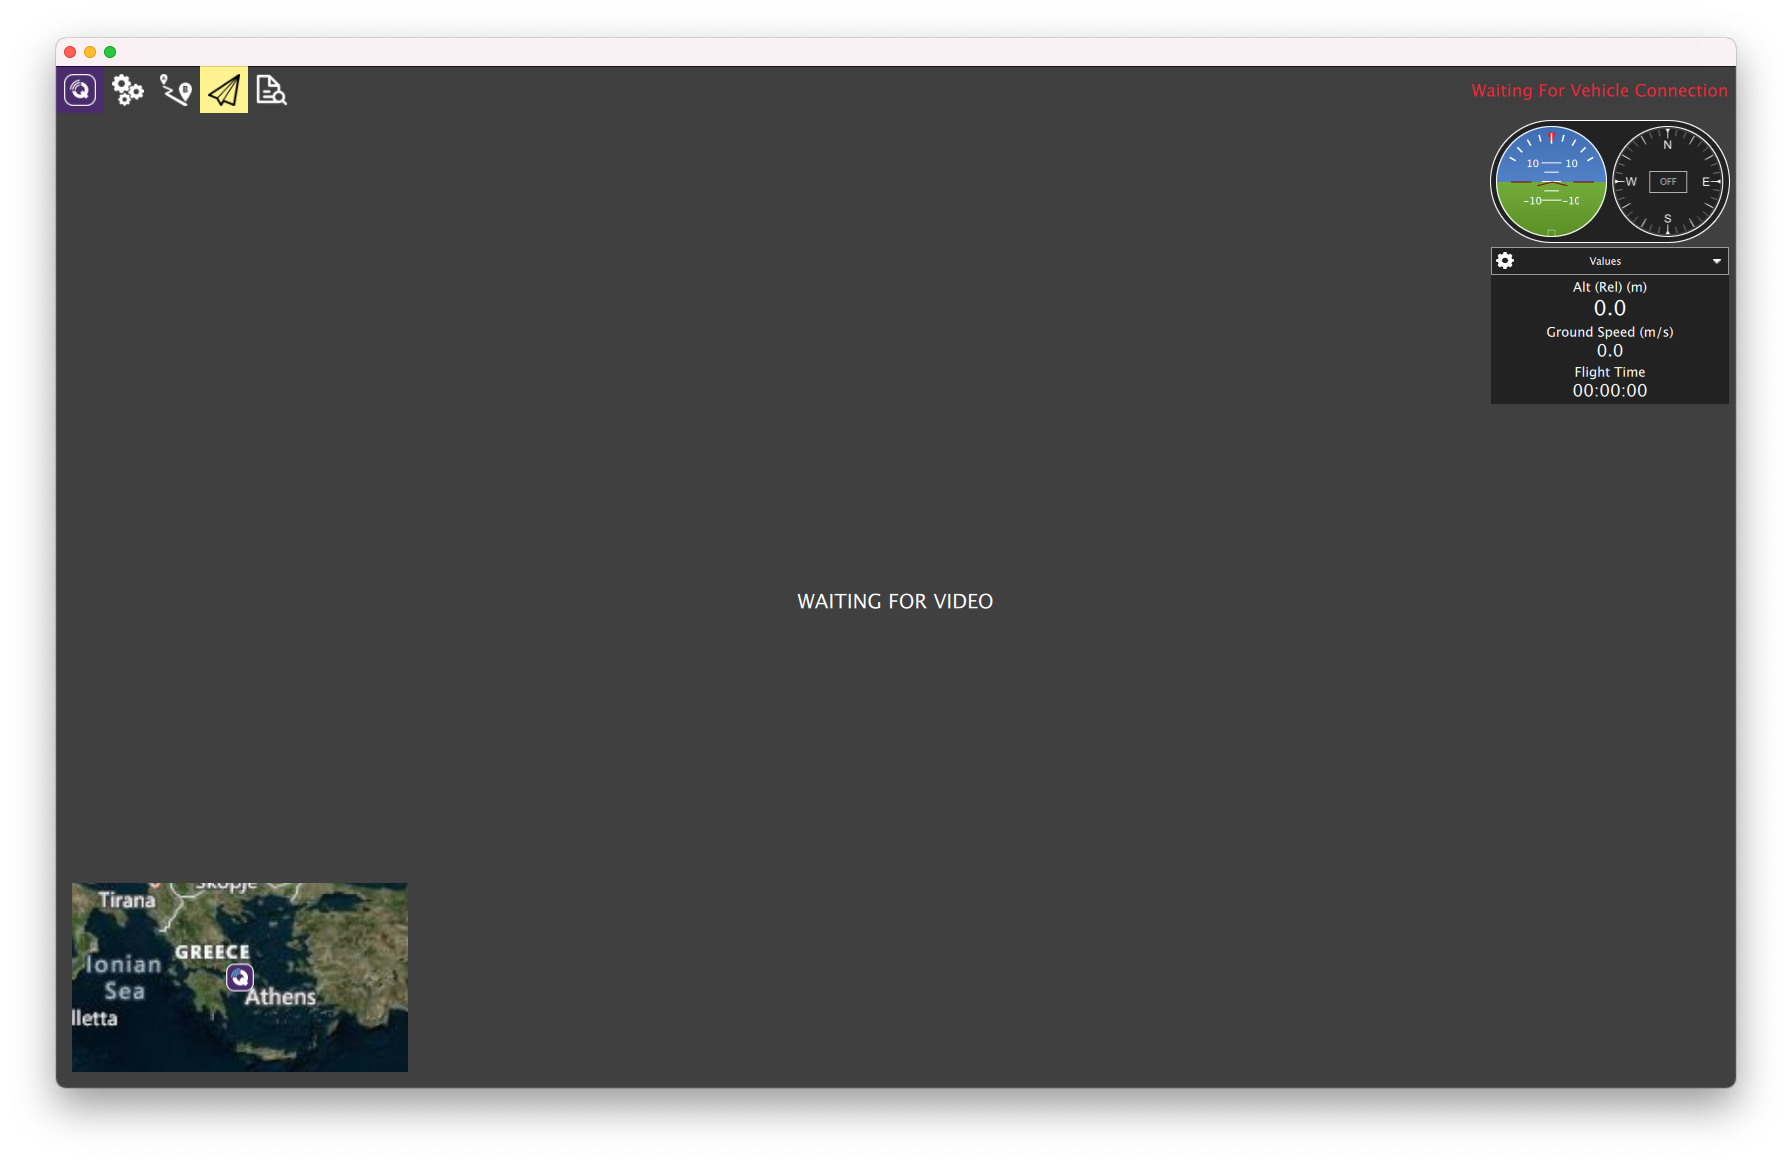
\includegraphics[width=1\textwidth]{templates/images/chapter05/qgc-before.png}
        \caption{Default Ground Control Station software state.}[Bottom row displays the request to allow traffic through the MAVLink port and the resulting information.]
        \end{minipage}
        
        \begin{minipage}{0.3\textwidth}
            \centering
            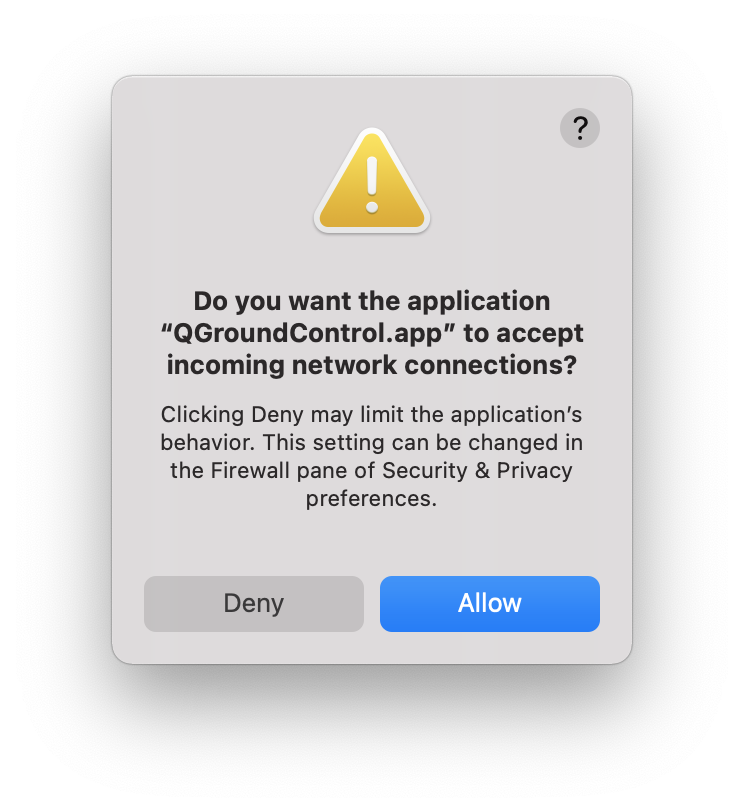
\includegraphics[width=\textwidth]{templates/images/chapter05/open-port.png} % first figure itself
            %\caption{Establish connection through the MAVLink protocol.}
        \end{minipage}\hfill
        \begin{minipage}{0.7\textwidth}
            \centering
            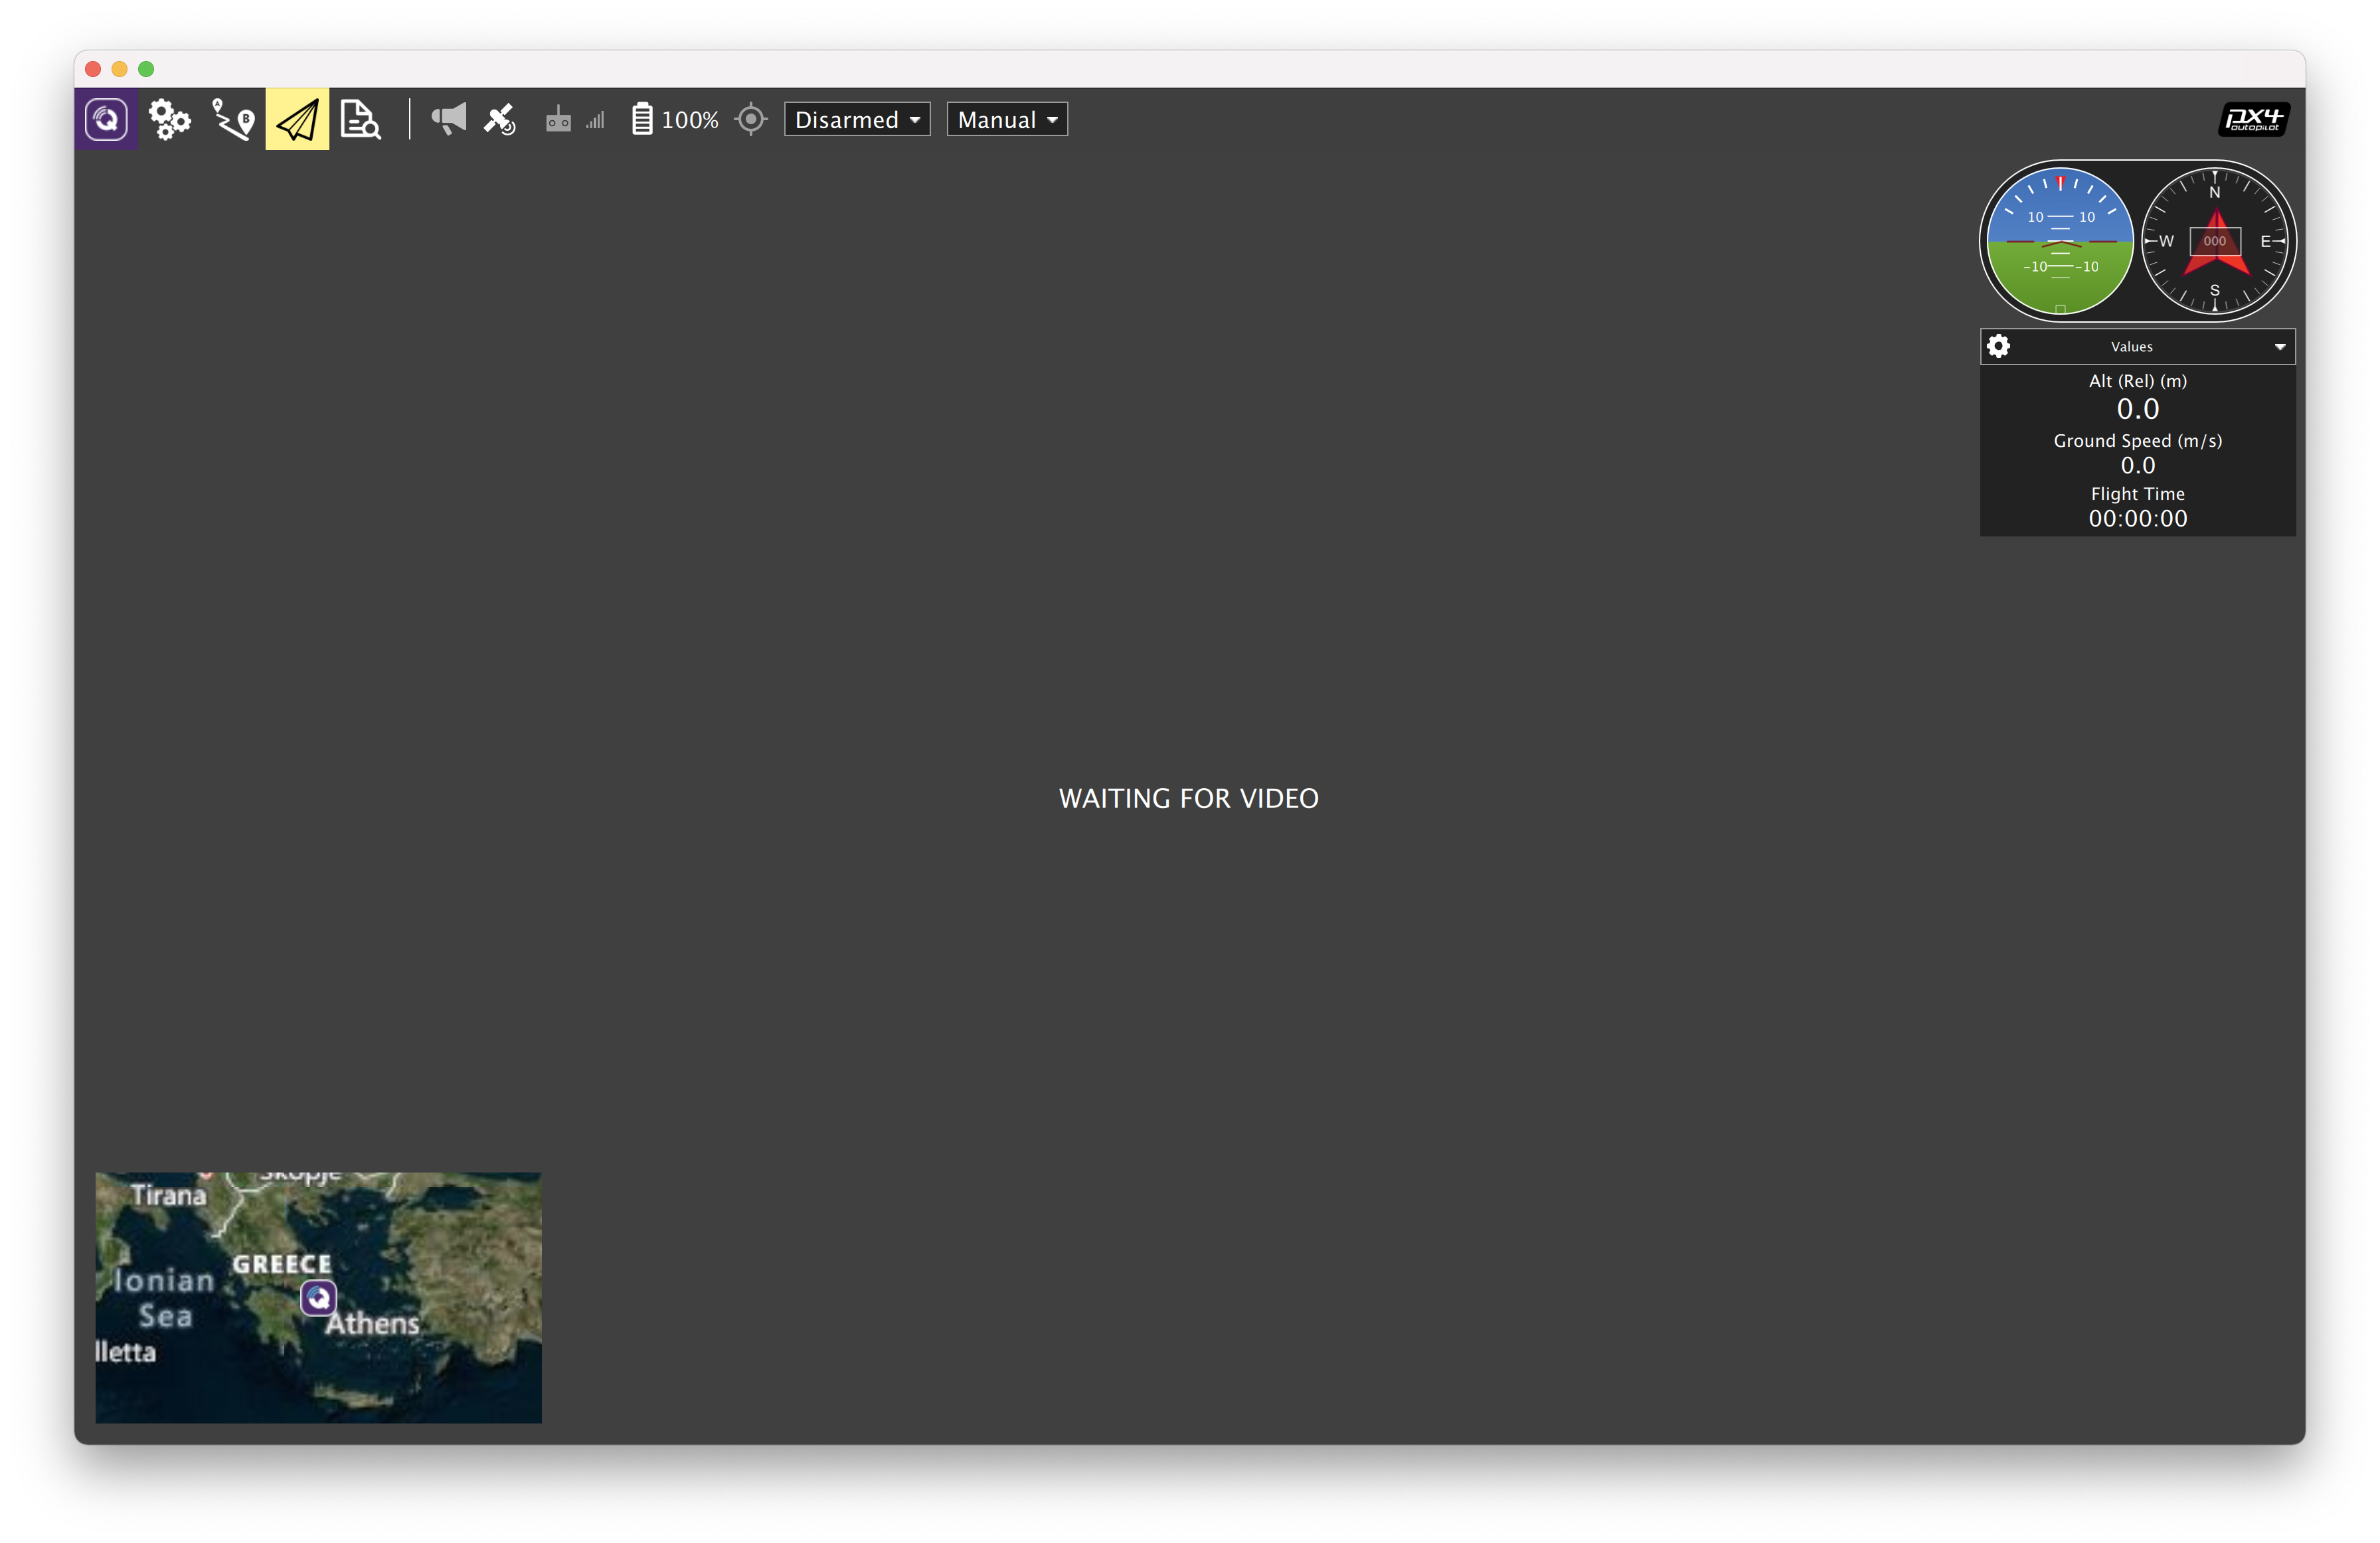
\includegraphics[width=\textwidth]{templates/images/chapter05/waiting-for-video.png} % second figure itself
            %\caption{Autopilot flight stack successfully connected.}
        \end{minipage}
        %\caption{Ground Station perspective after successful network connection.}
    \end{figure}
    
\newpage
    
    \subsubsection{Intel Camera Streaming Daemon}

    Camera streaming daemon gets installed with aero-system by default. It is responsible for detecting installed camera devices and proposing RTSP feeds. No further manual configuration is required.

    \begin{lstlisting}[caption=Check that CSD is running][H]
$systemctl status csd
csd.service - Camera Streaming Daemon
Loaded: loaded (/lib/systemd/system/csd.service; disabled; vendor preset: enabled)
Active: active (running) <output ommited>
    \end{lstlisting}
    
     Camera Streaming Daemon will stream the video feeds over the network with RTSP, a standard protocol. RTSP video can be received by QGroundControl and typical video players on most platforms.
    
    Intel Aero is proposing by default 5 RTSP video feeds:
    \begin{lstlisting}
RealSense R200, HD camera: rtsp://192.168.8.1:8554/video13
RealSense R200, depth sensor: rtsp://192.168.8.1:8554/rsdepth
RealSense R200, infrared first camera: rtsp://192.168.8.1:8554/rsir
RealSense R200, infrared second camera: rtsp://192.168.8.1:8554/rsir2
Bottom facing global shutter: rtsp://192.168.8.1:8554/bottom
    \end{lstlisting}
    
        \begin{figure}[!ht]
            \centering
            \includegraphics[width=0.4\textwidth]{templates/images/chapter05/rtsp-stream.png}
            \caption{RTSP video stream of the front-facing camera.}
            \label{fig:board-diagram}
        \end{figure} 
    
%    \subsubsection{gstreamer}
%        We covered the Camera Streaming Daemon to stream RTSP feeds. But you can also use gstreamer directly to encode (using the GPU) and send video over the network, drastically improving video latency over VLC. 
%<*own example>
%        Here an example using Yocto, launching a gstreamer command to get video from the RGB sensor of the R200 camera (/dev/video13), select a VGA resolution at 15fps, use the hardware accelerated h264 encoder and send it to a specific IP address:
%       \begin{lstlisting}
%sudo gst-launch-1.0 v4l2src  device=/dev/video13 do-timestamp=true ! video/x-raw, format=YUY2, width=640, height=480, framerate=15/1 ! autovideoconvert ! vaapih264enc ! rtph264pay !  udpsink host=192.168.1.147 port=5600
%        \end{lstlisting}

\newpage 
    \begin{figure}[H]
        \centering
        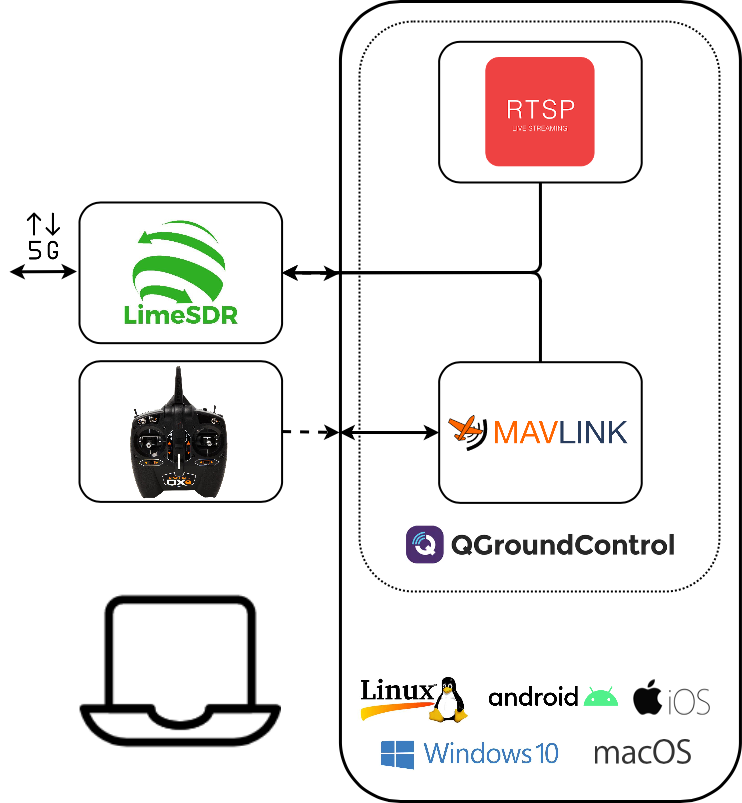
\includegraphics[width=0.9\textwidth]{templates/images/chapter05/user-side-overview-3.png}
        \caption{User-side overview of the software sub-systems.}
        \label{fig:board-diagram}
    \end{figure} 

        \subsubsection{QGroundControl}
        QGroundControl provides full flight control and vehicle setup for PX4 or ArduPilot powered vehicles. It provides easy and straightforward usage for beginners, while still delivering high end feature support for experienced users. The MAVLink "microservices" define higher-level protocols that MAVLink systems can adopt in order to better inter-operateand are used to exchange many types of data, including: parameters, missions, trajectories, images and other files.

        \begin{figure}[H]
            \centering
            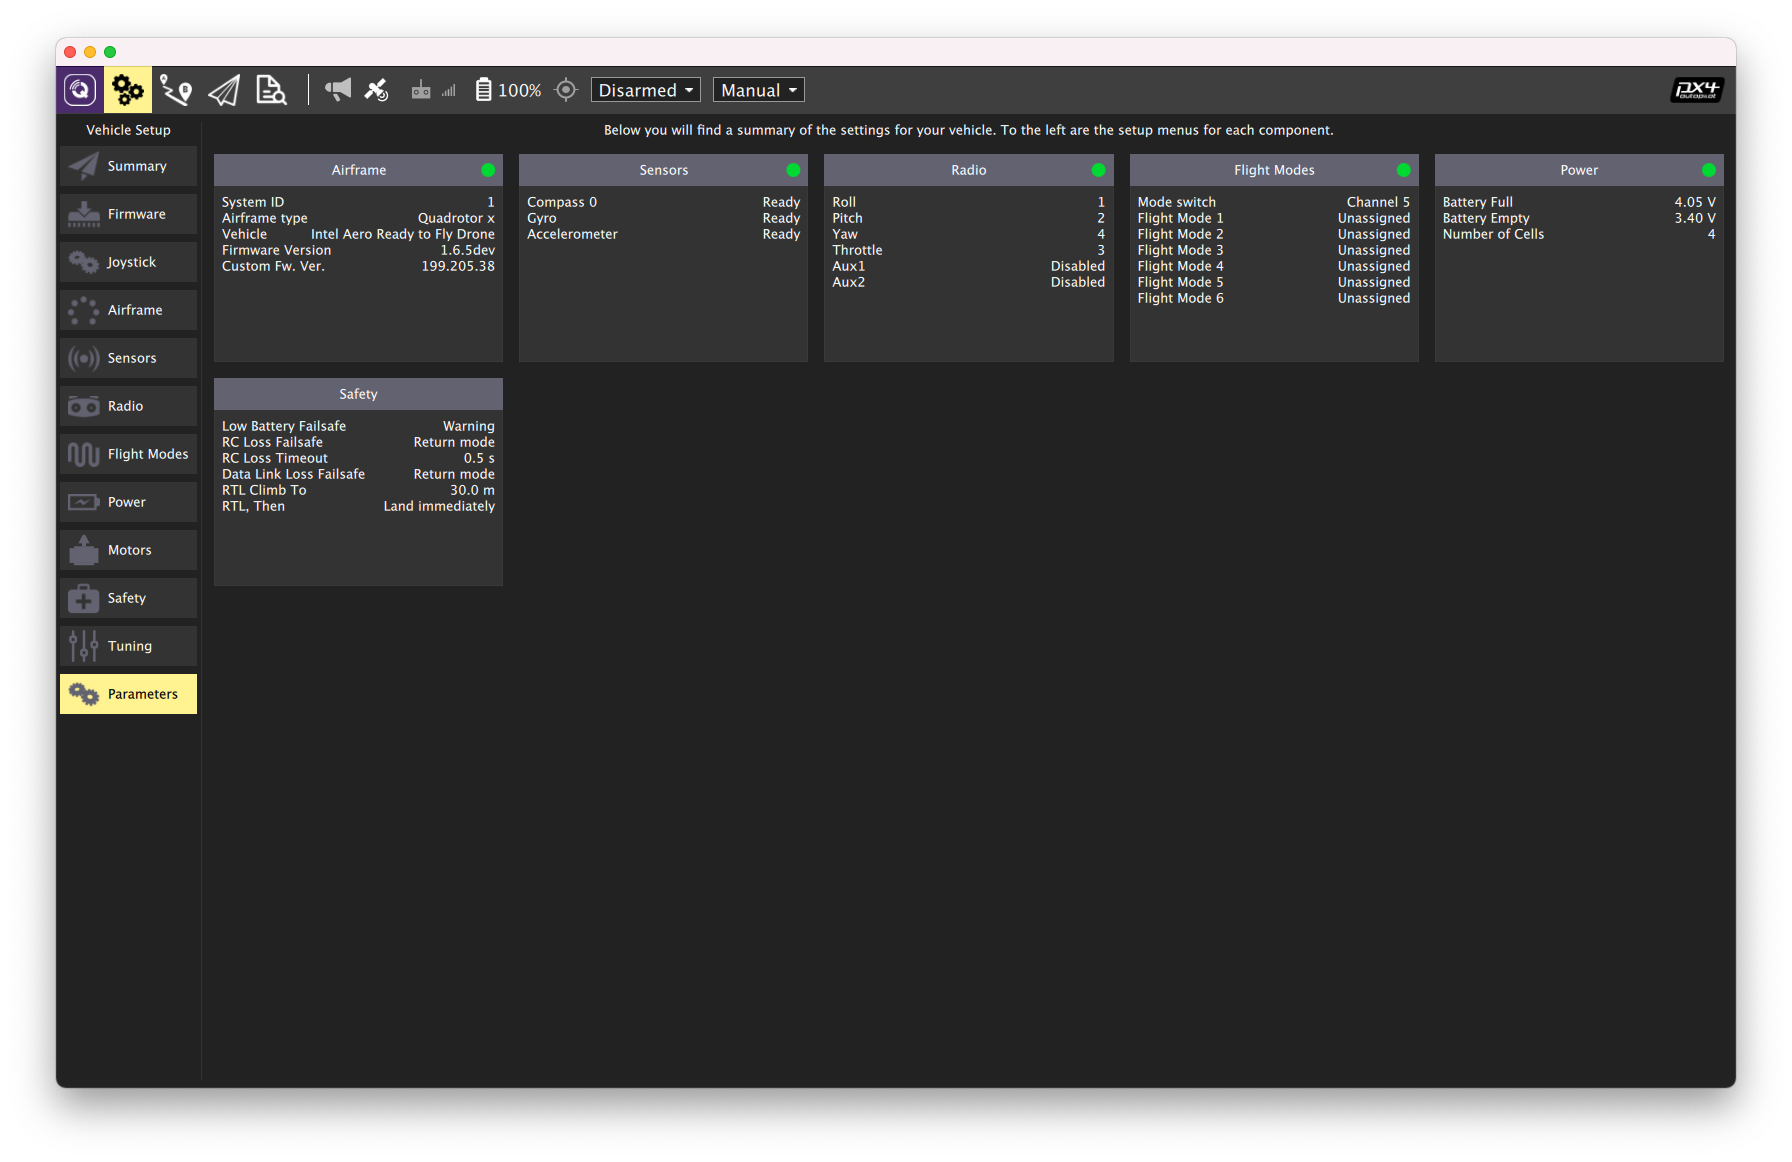
\includegraphics[width=0.9\textwidth]{templates/images/chapter05/passing-all-checks-to-arm-motors.png}
            \caption{Result of proper calibration of all sensors to arm motors.}
            \label{fig:board-diagram}
        \end{figure} 
        
        \begin{figure}[H]
            \centering
            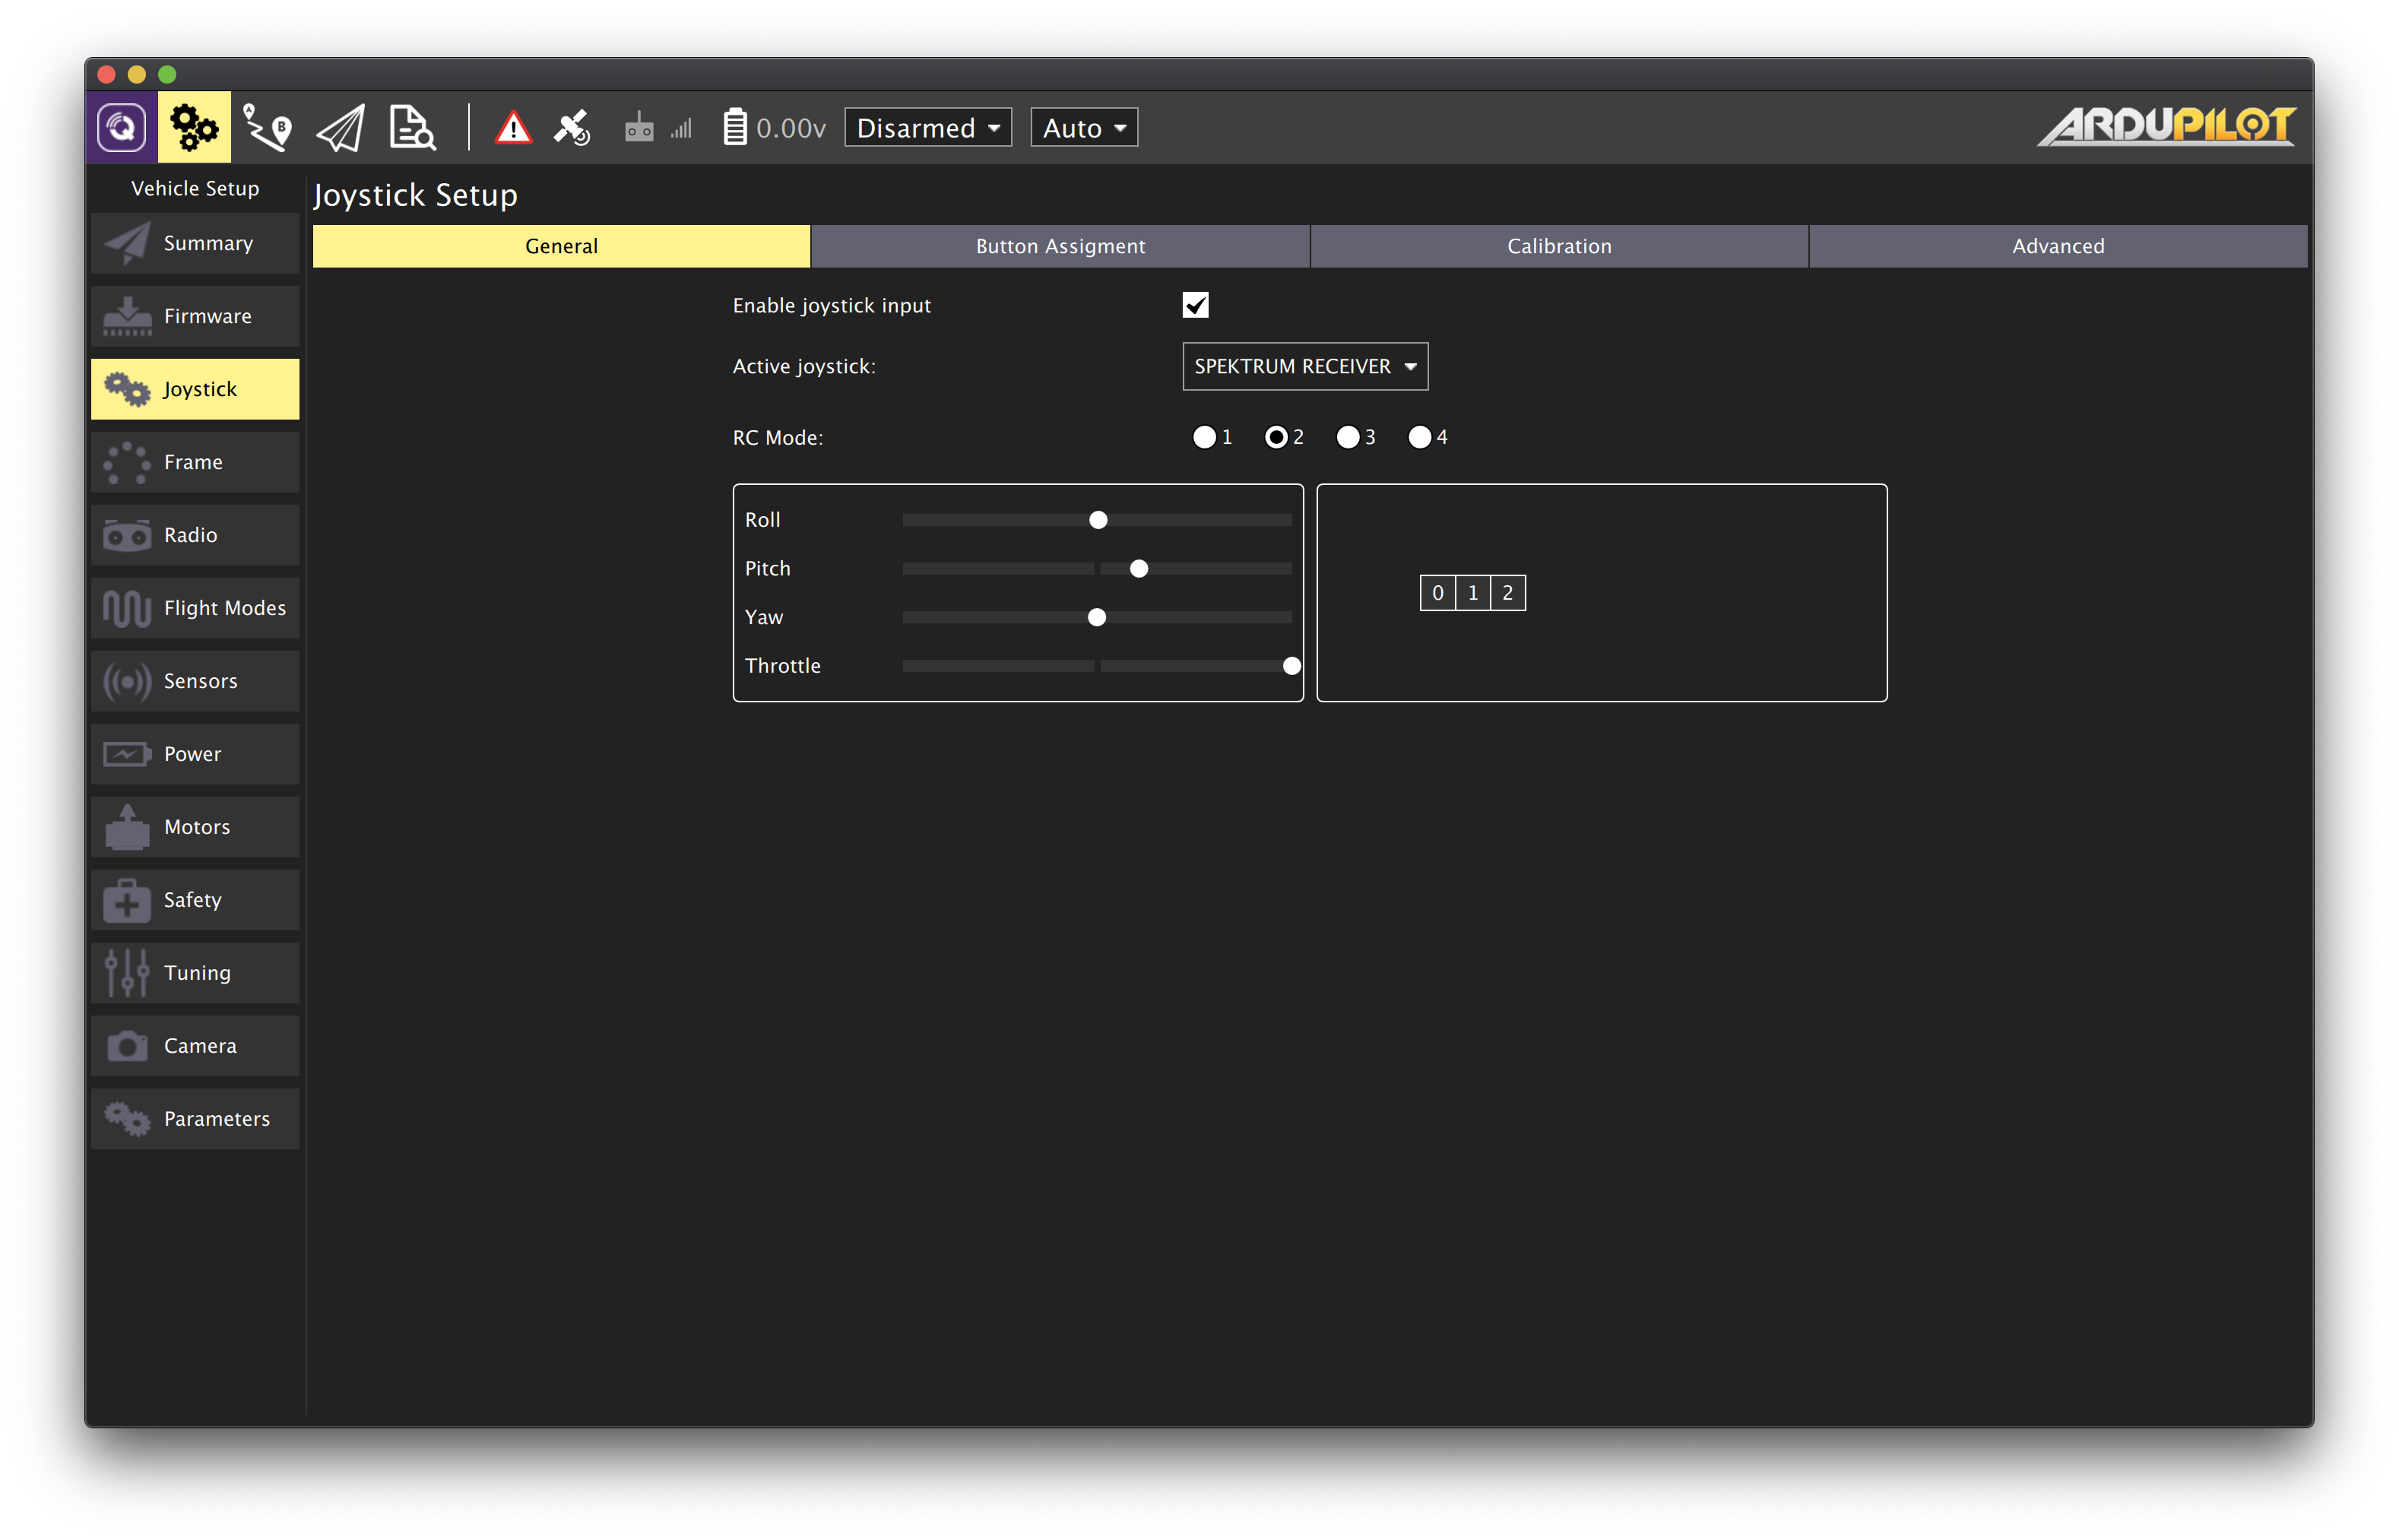
\includegraphics[width=0.9\textwidth]{templates/images/chapter05/joystick-setup-general.png}
            \caption{Verifying wireless controller adapter is recognized as input.}
            \label{fig:board-diagram}
        \end{figure} 
        
        \begin{figure}[H]
            \centering
            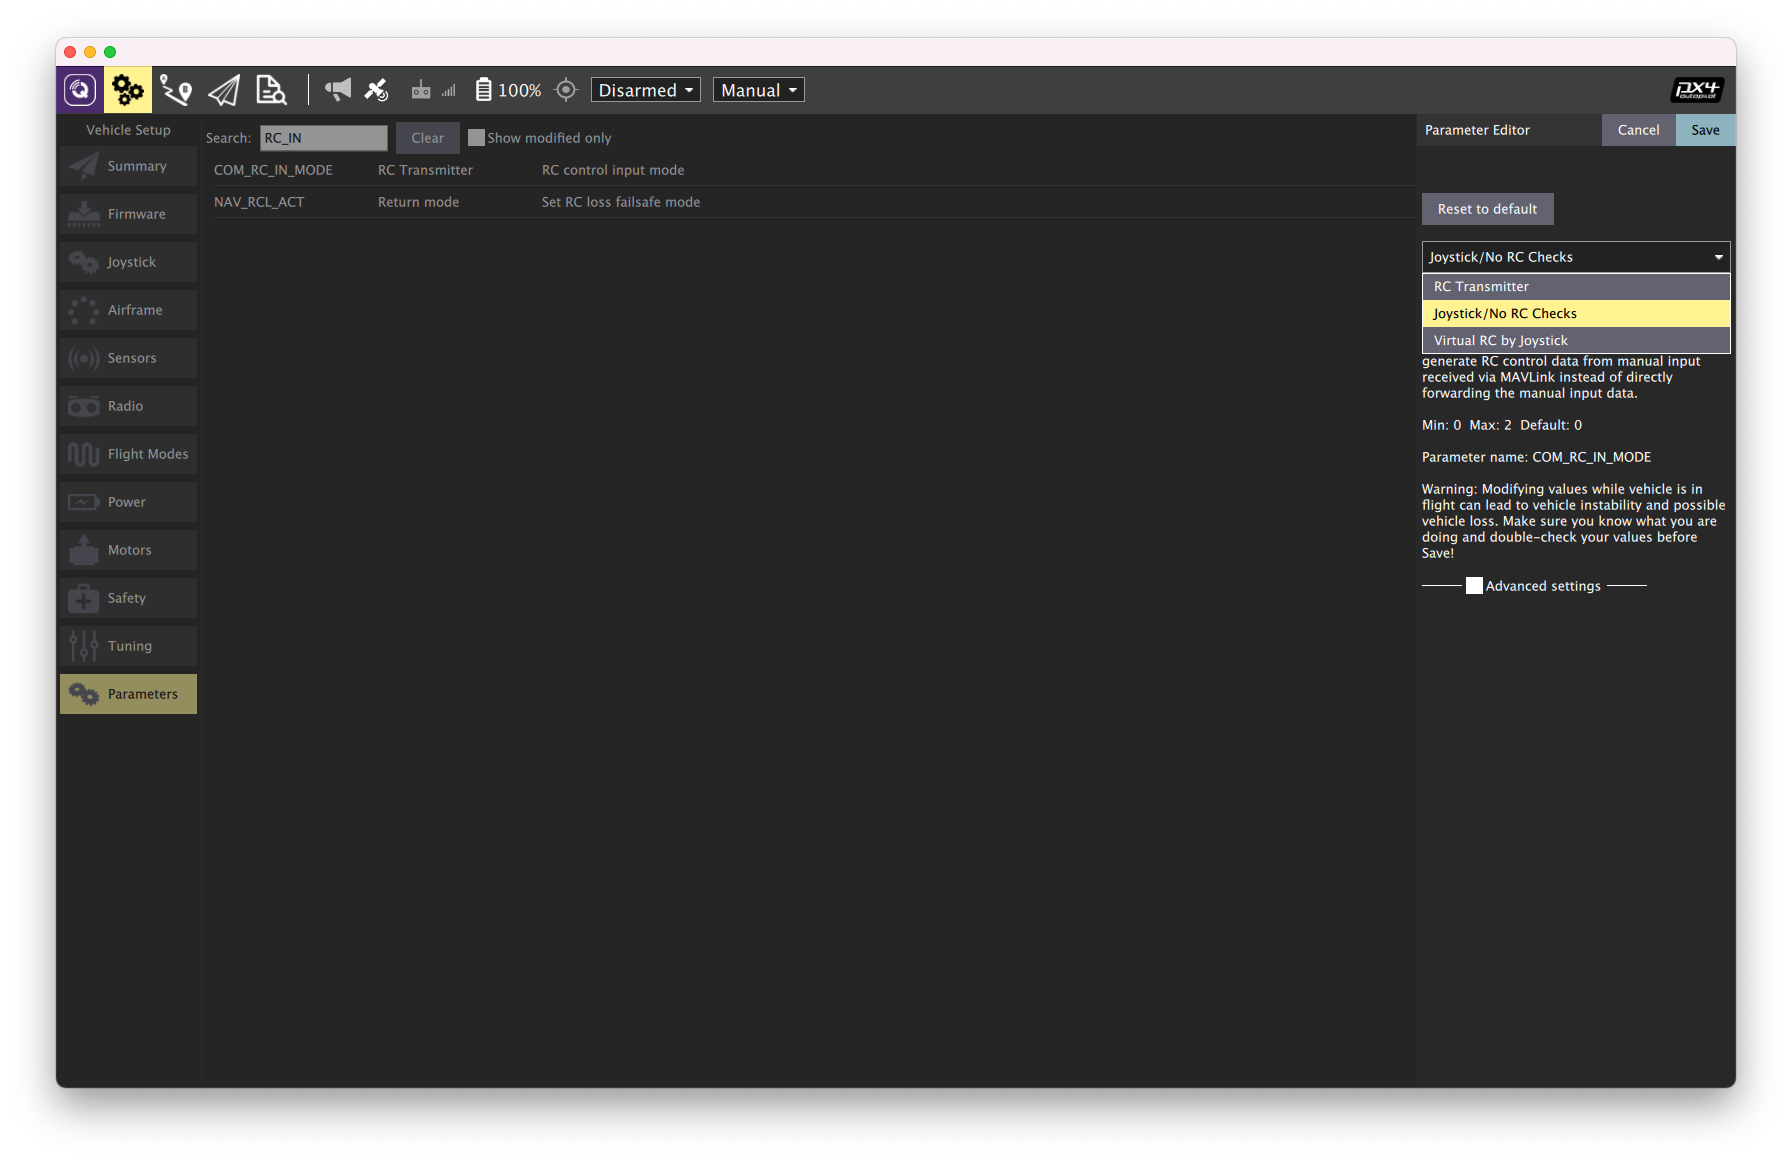
\includegraphics[width=0.9\textwidth]{templates/images/chapter05/setting-joystick-as-input.png}
            \caption{Setting parameter COM\_RC\_IN\_MODE to accept Joystick input.}
            \label{fig:board-diagram}
        \end{figure}
%\newpage
        By default, QGC communicates directly with Aero when connected to the same subnet. However, when the drone is on a cellular connection, a direct connection is non-trivial as both the drone and PC can be behind multiple layers of NATs/firewall. In the options described below, a cloud server is used to help route packets between the drone and PC. Alternatively, the prospective MEC of the gNodeB would be a prime candidate for hosting said instances for greatly reduced latency, as seen on Figure \ref{fig:mav-router}. %MEC of the facility

        On the Intel Aero Ready to Fly Drone (aka Aero RTF), mavlink-router runs locally to handle routing packets between the flight controller and different IP endpoints. But we can also deploy another instance of mavlink-router in the cloud to handle routing just IP traffic. Both the drone and QGC are then connected to this cloud based mavlink-router and communication is established. One benefit of using this method is flight logs are stored automatically in the cloud, so a copy of the logs can always be retrieved. This method also scales well with one-to-many use cases.
        
        \begin{figure}[H]
            \centering
            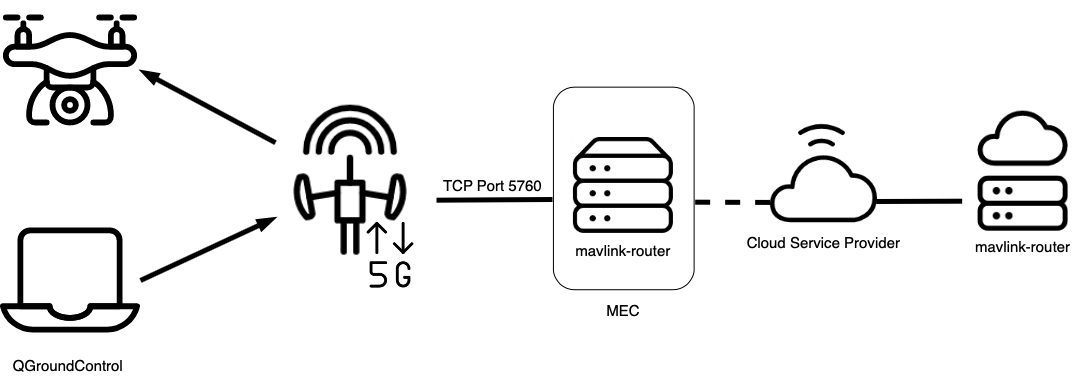
\includegraphics[width=0.9\textwidth]{templates/images/chapter05/mavlink-router.png}
            \caption{MAVLink Router implementation}
            \label{fig:mav-router}
        \end{figure}
%https://github.com/intel-aero/meta-intel-aero/wiki/91-(References)-LTE-Modems#qgroundcontrol-over-lte

        \begin{lstlisting}[caption=Check that MAVLink Router is running]
#Check if the system is listening for MAVLink messages on port 5760:
$netstat -l|grep 5760|
tcp        0      0 *:5760              *:*           LISTEN
        \end{lstlisting}
        
            \begin{figure}[!ht]
                \centering
                \includegraphics[width=0.9\textwidth]{templates/images/chapter05/final-look-QGC.png}
                \caption{Complete view of the Ground Control Station software.}
                \label{fig:board-diagram}
            \end{figure} 
    
\section{Networking}
%    \subsection{WiFi}
    By default, Intel Aero is networking through WiFi, either as a client or host. This is especially useful during development periods and short-range tests. Throughout the duration of this work, WiFi connectivity was used for testing purposes, with cellular connectivity roll-out planned for later stages. Regardless, few things are expected to differ in terms of configuration and overall setup.
    
%\subsection{Cellular}
    The Intel Aero Compute Board enables LTE modem devices to be installed into the M.2 interface by implementing a modem management software in the updated BIOS, especially convenient for our intended use-case, as any future M.2 form-factor modems can be swapped out, thus allowing easier connectivity upgrades and testing.
        
    \begin{enumerate}
        \item The modem will be installed into the M.2 connector which is located on the top side of the Aero Compute Board, adjacent to the 80 pin I/O  Connector. 
        
        \item When installing the modem, two antennas are required for proper operation. The WiFi antennas could be re-purposed for use with the LTE modem, but since both functions are required, we will be adding antennas which will extend the range of the drone's cellular radio.
        
        %\item The SIM card slot is located on the bottom side of the Compute Board underneath the 80 pin I/O Expansion Connector.

        \item Modem Manager should automatically detect the installed LTE modem and enumerate it as Modem 0 with \verb|$mmcli -m 0|. An APN must be set appropriately to access the network. %In order to show the details of the assigned IP addresses: \verb| $mmcli -b <bearer number>|
    \end{enumerate}

    \begin{figure}[H]
    \centering
    \begin{minipage}{0.48\textwidth}
        \centering
        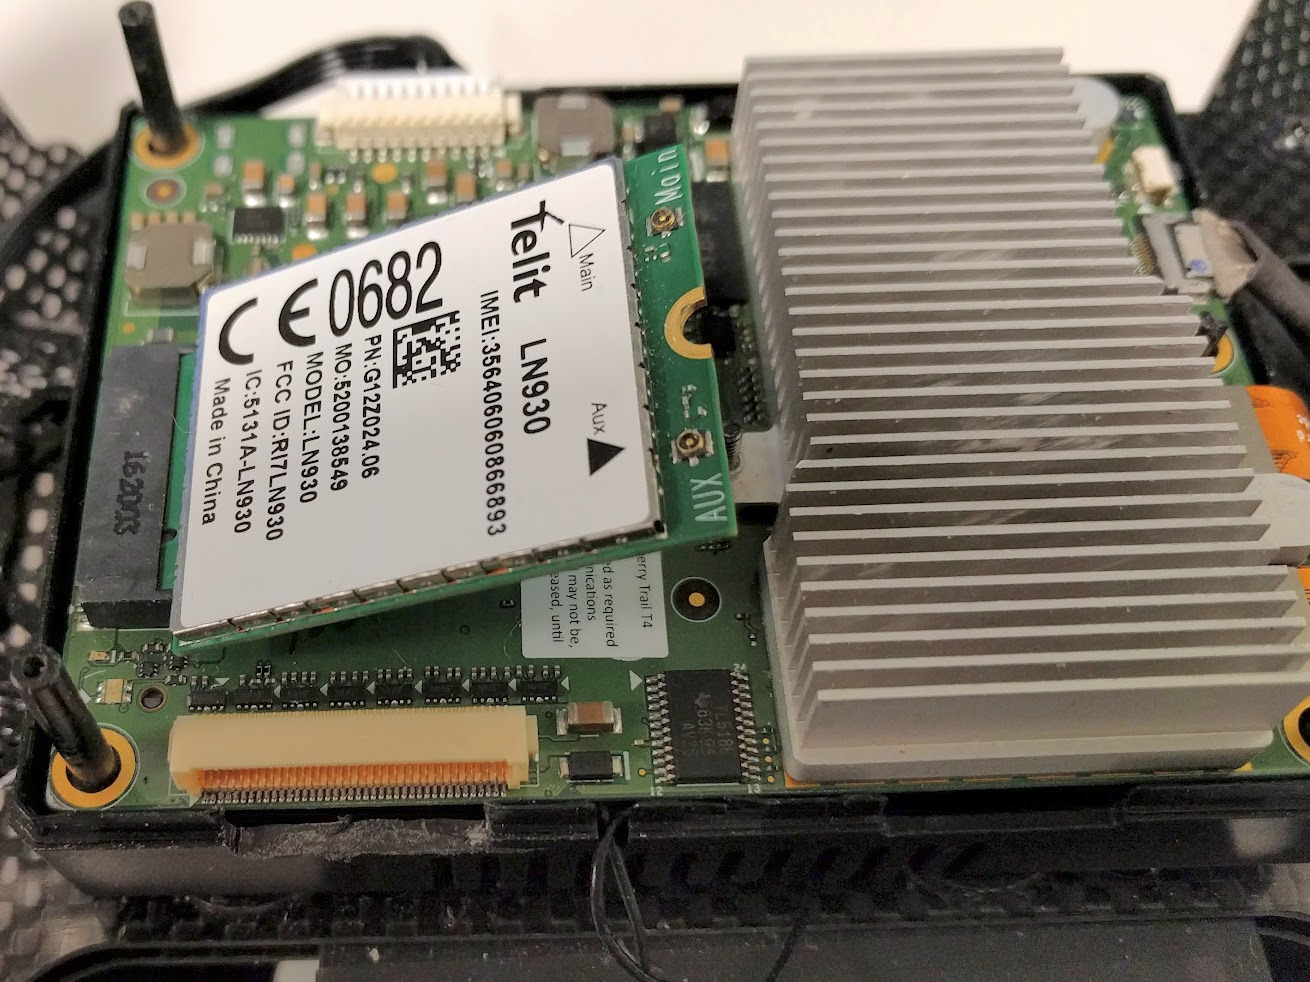
\includegraphics[width=\textwidth]{templates/images/chapter05/modem-insert-a.png} % first figure itself
        %\caption{first figure}
    \end{minipage}\hfill
    \begin{minipage}{0.48\textwidth}
        \centering
        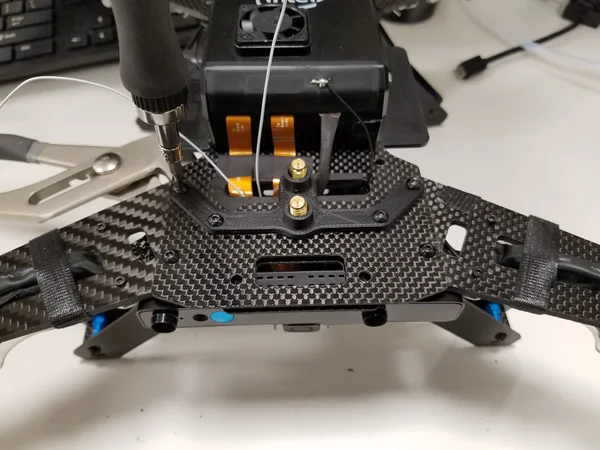
\includegraphics[width=\textwidth]{templates/images/chapter05/range-extender.png} % second figure itself
        %\caption{second figure}
    \end{minipage}
    \caption{Installing the modem and placing the additional antenna mounts.}
    \end{figure}

\section{Docker and Container Networking}

    There are many benefits for abstracting from a typical desktop OS installation in our specific use-case. A major one would be the compartmentalization of each of the processes that is to be run isolated from each other, as to ensure proper resource allocation, alleviating at the same time dependency problems previously mentioned. In this way, by updating only the docker runtime environment, each process can be install, updated and run independently. An added benefit of this setups would be of course its evolution to interact with the next-generation capabilities of 5G Core (or any next-gen network for that matter). By this, each initialized instance would be able to request a specific type of network slice according to its use, all the while providing added benefits of load balancing and fault tolerance that are eclipsed from regular OS or VM implementations.
    
    Following, are the three main docker container images that will be supplied with the finalized version of this drone platform, each geared towards a specific purpose in the overall use-case scenario.

    \subsection{srsue}
    
    srsLTE is a free and open-source LTE software suite developed by SRS %(www.softwareradiosystems.com). 
    The srsUE, srsENB and srsEPC applications include example configuration files that should be modified to meet the system configuration. Running the command \verb|sudo srsue| and by using the default configuration, creates a virtual network interface named "tun\_srsue" on the container with an IP in the network 172.16.0.x. Assuming the UE has been assigned an IP, we may now theoretically exchange traffic over the cellular link.
%https://github.com/srsLTE/srsLTE
    
    By default, containers are attached to a Docker network with a default route. This means everyone has internet access through the virtualized Docker network. In our use-case, the default-route parameter should be modified to point towards the \verb|srsue| container, which will handle the software stack that establishes the cellular connection either through a conventional modem or software-defined radio device. In order to make containers access the internet through the \verb|srsue| instead, we simply: 
    \begin{itemize}
    \item Configure network address translation at the UE
    \begin{lstlisting}
    docker exec virtual-srsepc iptables -t nat \
    -A POSTROUTING -s 172.16.0.0/24 -o eth0 -j MASQUERADE
    \end{lstlisting} This will masquerade all forwarded traffic from local containers (matched by source IP address) leaving the UE's eth0 (Docker) interface.
    
    \item Configure microservices containers to route traffic via the srsue by default

    \verb|docker exec virtual-srsue ip route replace default via 172.16.0.1|
    
    \end{itemize}
    Now we should have network access through the onboard UE software stack.
%[https://github.com/pgorczak/srslte-docker-emulated]
    
    Additionally, the library currently supports the Ettus Universal Hardware Driver (UHD) and the bladeRF driver. Thus, any hardware supported by UHD or bladeRF can be used, assuming allocation to the appropriate container. There is no sampling rate conversion, therefore the hardware should support 30.72 MHz clock in order to work correctly with LTE sampling frequencies and decode signals from live LTE base stations.
    
    %FDD and TDD configuration, Carrier Aggregation support, Cell search and synchronization procedure for the UE, Soft USIM supporting Milenage and XOR authentication, Hard USIM support using PCSC framework, Virtual network interface tun\_srsue created upon network attach
    %https://github.com/srsLTE/srsLTE

    \subsection{gstreamer}

    Due to poor streaming quality and performance by using conventional network feed streaming applications such as VLC, another solution would need to be implemented in order to further reduce the latency of the video transmission. For this reason, gstreamer, an open-source multimedia framework, is able to provide the granularity that's required in our use-case. Examples of that include -but are not limited- to enabling H.264 encoding, target frametime, resolution and aspect ratio, aswell as accepting multiple inputs at the same time. By configuring the appropriate default gateway setting on the networking parameters of this container and exposing its relevant network ports, we should be able to override using the system's bridge network and route the rtsp stream through \verb|srsue|.
    
%\newpage

    \subsection{mavlink-router}

    As previously mentioned, mavlink-router's sole purpose is to provide an encapsulation method for MAVLink packets to traverse the IP network. Additionally, its versatility in terms of addressing also provides a strategic advantage in terms of flexibility, as it can route streams to and from multiple devices independently at the same time. For this reason, by creating a basic container image and pointing the ttyS1 serial device to it, each running image will be able to handle separately traffic between the flight controller and ground station end points. Same as before, we can route the connectivity of the MAVLink messages through the software stack of \verb|srsue|.

%\newpage 

%The type of network a container uses, whether it is a bridge, an overlay, a macvlan network, or a custom network plugin, is transparent from within the container. From the container’s point of view, it has a network interface with an IP address, a gateway, a routing table, DNS services, and other networking details (assuming the container is not using the none network driver). This topic is about networking concerns from the point of view of the container. By default, when you create or run a container using docker create or docker run, it does not publish any of its ports to the outside world. To make a port available to services outside of Docker, or to Docker containers which are not connected to the container’s network, use the --publish or -p flag. This creates a firewall rule which maps a container port to a port on the Docker host to the outside world.

%    By default, the container is assigned an IP address for every Docker network it connects to. The IP address is assigned from the pool assigned to the network, so the Docker daemon effectively acts as a DHCP server for each container. Each network also has a default subnet mask and gateway. When the container starts, it can only be connected to a single network, using --network. However, you can connect a running container to multiple networks using docker network connect. When you start a container using the --network flag, you can specify the IP address assigned to the container on that network.
%https://docs.docker.com/config/containers/container-networking/
%    In terms of networking, a bridge network is a Link Layer device which forwards traffic between network segments. A bridge can be a hardware device or a software device running within a host machine’s kernel. In terms of Docker, a bridge network uses a software bridge which allows containers connected to the same bridge network to communicate, while providing isolation from containers which are not connected to that bridge network. The Docker bridge driver automatically installs rules in the host machine so that containers on different bridge networks cannot communicate directly with each other. Bridge networks apply to containers running on the same Docker daemon host. When you start Docker, a default bridge network (also called bridge) is created automatically, and newly-started containers connect to it unless otherwise specified. Containers on the default bridge network can only access each other by IP addresses, unless you use the --link option, which is considered legacy. All containers without a --network specified, are attached to the default bridge network. This can be a risk, as unrelated stacks/services/containers are then able to communicate. Using a user-defined network provides a scoped network in which only containers attached to that network are able to communicate by enterind the command \verb|$ docker network create my-net|.
%    You can specify the subnet, the IP address range, the gateway, and other options. When you create or remove a user-defined bridge or connect or disconnect a container from a user-defined bridge, Docker uses tools specific to the operating system to manage the underlying network infrastructure (such as adding or removing bridge devices or configuring iptables rules on Linux).
%https://docs.docker.com/network/bridge/ 